\documentclass[11pt, a4paper]{article}

\usepackage[lang=en,grid=dark]{kufront}

\usepackage{tikz}
\usetikzlibrary{shapes,matrix}
\usepackage[utf8]{inputenc}
\usepackage{amsmath, amssymb}
\usepackage{mathtools}
\usepackage{amsfonts}
\usepackage{pdfpages}
\usepackage{gauss}
\usepackage{fancyvrb}
\usepackage{hyperref}
\usepackage{graphicx}
\usepackage{subcaption}
\usepackage{url}
\usepackage{float}
\usepackage[bottom]{footmisc}
\usepackage{color}

% algorithms
\usepackage{algorithm}              % algorithm float environment
\usepackage[noend]{algpseudocode}   % from algorithmicx; no "end" on functions
\newcommand*\Let[2]{\State #1 $\gets$ #2}
\algrenewcommand\algorithmicrequire{\textbf{Precondition:}}

% headers and footers
\usepackage{fancyhdr, lastpage}
\pagestyle{fancy}
\fancyhf{}
\renewcommand{\headrulewidth}{0pt}
\cfoot{Page \thepage\ of~\pageref{LastPage}}

% settings for lslisting
\definecolor{listinggray}{gray}{0.9}
\usepackage{listings}
\lstset{
  %backgroundcolor=\color{listinggray},
  %tabsize=2,
  %rulecolor=,
  %frame=single,
  showtabs=false,
  showspaces=false,
  showstringspaces=false,
  columns=fixed,
  showstringspaces=false,
  extendedchars=true,
  %identifierstyle=\ttfamily,
  %keywordstyle=\color[rgb]{0,0,1},
  %commentstyle=\color[rgb]{0.133,0.545,0.133},
  %stringstyle=\color[rgb]{0.627,0.126,0.941},
  %literate={\$}{{\textcolor{blue}{\$}}}1,
  %breaklines=false,
  %prebreak=\raisebox{0ex}[0ex][0ex]{\ensuremath{\hookleftarrow}},
  %breakatwhitespace=false,
}

\lstdefinestyle{output-style}{
  basicstyle=\ttfamily\footnotesize,
  frame=tb,
  %xleftmargin=10em
}

% handy commands etc.
\newcommand{\eqdef}{\overset{\mathrm{def}}{=\joinrel=}}

\title{Efficient DNA/RNA sequence clustering}
\subtitle{Using $k$-mers as an approximation\\for sequence similarity}
\author{Anders Kiel Hovgaard \& Nikolaj Dybdahl Rathcke}
\date{June 8, 2015}
\project{Bachelor's Thesis}
\supervisor{Supervisor: Rasmus Fonseca \& Martin Asser Hansen}

\begin{document}
\begin{titlepage}
  \maketitle
\end{titlepage}

\begin{abstract}
  This will eventually contain a beautiful abstract \dots
\end{abstract}

\thispagestyle{plain}
\pagenumbering{roman}
\newpage

\tableofcontents
\thispagestyle{plain}
\newpage

\thispagestyle{fancy}
\pagenumbering{arabic}

\section{Introduction}

Clustering is the task of partitioning a set of objects, such that each
partition contains objects that are similar to each other and objects in
separate partitions are dissimilar, according to some well-defined notion of
similarity. These partitions are called \emph{clusters}.

Clustering huge amounts of DNA/RNA sequences (up to 500 million strings of
500--1500 characters each) is computationally hard, and the cost of sequencing,
i.e. determining DNA and RNA data, has dropped so low, and consequently the
amount of data has grown so large, that the available algorithms and hardware
can no longer keep up.~\cite{rothberg}

There are not many available algorithms and tools for efficient clustering of
sequencing data. The one tool which is currently doing the job,
\texttt{USEARCH}~\cite{edgar, usearch}, is closed-source and although the
32-bit version is available for free, the usable memory is limited to 4 GB and
the 64-bit version is costly.

As the amount of sequencing data grows, clusterings becomes increasingly more
relevant as it can be used to reduce a large set of sequences to a much smaller
set of representative sequences, called \emph{centroids}, which each represents
a single cluster.

This project is concerned with the clustering of DNA and RNA sequences. The
clustering method described in this document strives to assign each sequence to
a cluster based on the similarity between the sequence and the centroid. The
clustering method does not guarantee a minimal number of clusters, as the
search for a centroid is not exhaustive, nor does it guarantee to find the most
similar centroid for each sequence. The clustering algorithm tries to minimize
the number of clusters.

This project researches the possibilities for creating an open-source tool that
can match the performance of \texttt{UCLUST}. We present a solution and
implementation that uses the concept of $k$-mer counting, i.e. essentially
comparing the distribution of all possible substrings of a fixed length $k$ in
each sequence, as an approximation for measuring sequence similarity.
Furthermore, it utilizes the $k$-mers occurring in the centroids for improving
the search for a centroid that is likely to be a good representative for a
given centroid.

Earlier works have been very focused on techniques based on sequence alignment,
with \texttt{UCLUST} being one such example. However, a clustering algorithm
with a similarity measure based on $k$-mers, can possible give an improved
performance in terms of speed, while still being a sufficiently good
approximation.

% TODO, maybe add joke: klust, or \texttt{$k$-lust} depending on your temper
Our program, named \texttt{klust}, has been implemented in \texttt{C++}, is
hosted on GitHub and is available at \url{https://github.com/Rathcke/klust}.

The reader of this document is expected to have a basic knowledge of computer
science, corresponding to around two or three years of undergraduate studies.

\section{Terminology}

The words \emph{sequence} and \emph{string} will be used to denote the same
concepts, i.e. an ordered list of objects, where an object will most often be a
text character. In general, a sequence or string might be infinite, but in this
project they will always be finite unless mentioned otherwise.

In this text, the notion of a subsequence is different from that of a
substring, as is the common convention: a \emph{substring} of a sequence $S$ is
a consecutive, ordered list of objects, that occurs in $S$, while a
\emph{subsequence} of $S$ is a sequence that can be obtained from $S$ by
deleting some objects from the sequence without changing the order of the
objects.

The \emph{distance} between sequences denotes some absolute measure of how far
the sequences are from each other in some well-defined space, e.g. which fixed
length substrings occur in the sequences and how many times.

The \emph{similarity} or \emph{identity} between sequences denotes a relative
measure of the distance between the sequences, i.e. a normalized distance
measure where 0 means no similarity and 1 means perfect similarity. A
\emph{similarity threshold} or \emph{identity threshold} is a similarity that
two sequences must have to belong in the same cluster.  When two sequences are
above a given similarity threshold, they are said to \emph{match} one another.

The terms \emph{query sequence} and \emph{target sequence} will be used to
denote the sequence being searched for and a sequence being compared to,
respectively.

The name \texttt{USEARCH} denotes both the piece of software developed by
Robert C. Edgar and the algorithm used in the program for searching for
sequences in some database, e.g. for searching for a centroid that is above a
given distance threshold of some sequence. The name \texttt{UCLUST} refers to
the clustering algorithm used in the \texttt{USEARCH} program.


\subsection{Notation}

Let $s$ and $t$ be sequences.
\begin{itemize}
  \item $d(s,t)$ denotes the distance between $s$ and $t$
  \item $|s|$ denotes the length of $s$
  \item $s \sqsubseteq t$ denotes that $s$ is a substring of $t$
  \item $J(A,B)$ denotes the Jaccard index, or Jaccard similarity coefficient,
    of sets $A$ and $B$
\end{itemize}

\section{Background}

\subsection{Biology}
\label{sec:biology}

DNA, deoxyribonucleic acid, is a polymeric molecule that consists of the four
chemically distinct nucleotides adenine (A), cytosine (C), guanine (G) and
thymine (T). RNA, ribonucleic acid, is also a polymeric molecule where the
nucleotide thymine is replaced by uracil (U). The nucleotides can be linked
together in any order to form chains that are up to millions of nucleotides
long~\cite[pp.~8--9]{brown}. These chains are called sequences.

Besides the four nucleotides in DNA and RNA, sequencing data can also contain
\emph{ambiguous bases} such as 'R', 'Y', 'K'. These are used in sequencing
data to indicate uncertainties about the actual nucleotides. The ambiguous bases
represent different subset of the four nucleotides and there exists one for
each subset~\cite{tao}.

Every organism has a genome that contains the biological information that is
needed to construct and maintain a living example of that organism. For humans
and most other cellular life forms, the genome is made up of DNA, but a few
viruses have RNA genomes~\cite[pp.~3--4]{brown}.

Genomes are changing over time as a result of continuous small-scale sequence
alterations. These are called \textit{mutations}. Mutations happen because of
DNA replication errors or from damaging effects of mutagens, such as chemicals
or radiation. The mutations can be \textit{point mutations} which are single
nucleotide edits. Others include deletions of a section in the DNA and
insertions, where one or more nucleotides are inserted into a new place in the
DNA~\cite[pp.~505--506]{brown}. Another type of mutation is when a segment is
moved from one part of the sequence to another. These segments are known as
\emph{transposable elements}~\cite{munoz}.

Clustering can serve to identify DNA or RNA sequences that has been mutated and
group mutated sequences of the same origin into the same cluster with just a
single representative sequence.
\section{Methods} \label{sec:methods}

\subsection{Distance metrics}

The following sections describe a range of different types of distance metrics,
that is, methods for measuring the distance between sequences.

\subsubsection{Edit distance}\label{sec:edit_distance}

One type of \emph{edit distance} is the \emph{Levenshtein
distance}~\cite{levenshtein}, which is a string metric for determining the
similarity between two sequences. It is defined to be the minimum number of
edits to transform the first sequence into the other~\cite[p.~52]{dong}.

The edit operations consists of \emph{insertions}, \emph{deletions} and
\emph{substitutions}. These operations are, respectively, inserting a letter,
removing a letter and changing one letter into another.

For example, the two sequences
\begin{center}
  \texttt{ACGT} \\
  \texttt{ACGGC}
\end{center}
would have a distance of 2 (e.g. substituting T for G and inserting a C).
However, there are some cases where the relevance of the distance is arguable.
Consider the sequences
\begin{center}
  \texttt{AACCGG} \\
  \texttt{CCAAGG}
\end{center}
with a distance of 4. The mutation could be seen as the substring \texttt{CC}
acting as a transposable element, which one might want to result in a low
distance.

A bottom-up dynamic programming version of the Levenshtein distance metric was
implemented and tested on real DNA/RNA data to evaluate its performance, and it
was clear that this algorithm is not suitable for large data sets, because it
would be infeasible to complete even a linear time clustering, in the number of
sequences to be clustered. The implementation could most likely be optimized
further, but because of the characteristics of an edit distance algorithm like
Levenshtein and because of the performance requirements for this project, it
was decided to not pursue further optimization and instead focus on other types
of algorithms. Furthermore, the Levenshtein distance penalizes occurrences of
transposable elements, i.e. it results in an
increased distance.

The Levenshtein distance can still be used for evaluation and benchmarking
against other metrics. The algorithm is attached in appendix
\ref{app:levenshtein_algorithm} and results from tests are shown in section
\ref{sec:results}.

As stated in~\cite[pp.~1--2]{andoni}, ``The worst-case running time known for
this problem has not improved in three decades (..)'', specifically it states
that the running time of Levenshtein is $\mathcal{O}(d^2)$, where $d$ is the
length of the two sequences, and $\mathcal{O}(d^2/\log_2(d))$ for a constant
size alphabet. It further supports the conclusion that the running time of the
Levenshtein algorithm is too poor for the large data sets of the problem
domain.

This lack of improvements of the performance of edit distance is one motivation
for the introduction of the concept of sequence alignment.


\subsubsection{Sequence alignment}

\emph{Sequence alignment} is used in bioinformatics to identify regions of
similarity by aligning the characters of two or more sequences in a certain
manner. Besides shifting a sequence to a side, gaps can be inserted between
characters as well. A gap is represented with '-' and it indicates an insertion
in one sequence or a deletion from another sequence. This is called an
\emph{indel}, which is a contraction of the first letters from insertion and
deletion. If it is not an indel and all characters in the column are the same,
then it is a match. Otherwise, it is a mismatch~\cite[pp.~135--136]{dong}.

\begin{figure}[H]
  \centering
  \verb+ATGCAACGA+ \\
  \verb+ |||  |||+ \\
  \verb+-TGCG-CGA+
  \caption{Sequence alignment of `ATGCAACGA' and `TGCGCGA'}
  \label{fig:seq_alignment}
\end{figure}

Figure \ref{fig:seq_alignment} displays an alignment of two sequences. In
column 0 is an indel, in columns 1--3 are matches, in column 4 is a mismatch
and so forth. The vertical bar characters in the middle line, indicate matches.

% TODO: describe Needleman-Wunch, Smither-Waterman, multiple alignment, 
% global vs local

Both \texttt{UCLUST} and the very recent project \texttt{VSEARCH} uses some
kind of sequence alignment for comparing sequences. \texttt{VSEARCH} uses a
parallelized version of the dynamic programming algorithm Needleman-Wunsch,
while \texttt{UCLUST} uses a heuristic procedure by default, but can be
instructed to use full dynamic programming with either the Needleman-Wunsch or
Smith-Waterman algorithm. However, this will make \texttt{UCLUST} much
slower~\cite{vsearch}. The heuristic algorithm used in \texttt{UCLUST} gives an
approximation of the optimal alignment for the purpose of increased
performance, but the alignment is not guaranteed to be optimal.

As opposed to \texttt{USEARCH}, \texttt{VSEARCH} is free and open-source
software and is designed for 64-bit processors, so it does not have the
limitation on usable memory that the free, 32-bit version of \texttt{USEARCH}
has.

Sequence alignment is still a computationally expensive operation and for
comparison of sequences with low similarity, the results of sequence alignment
are often poor. Additionally, as with the Levenshtein distance metric, sequence
alignment is very sensitive to the ordering of parts of sequences.
\emph{Alignment-free} sequence comparison methods strive to provide a measure
of sequence similarity while avoiding the costly computation that alignment
involves. Alignment-free comparison allows one to look at each of the sequences
independently, extracting some characteristics, or \emph{features}, of each
sequence and then comparing these characteristics. This can possibly reduce the
complexity of the comparison to linear time or better. One such alignment-free
method, is $k$-mer counting which will be presented and analyzed in the
following section.


\subsubsection{Feature based distance} \label{sec:kmer_distance}

A \emph{$k$-mer}, or \emph{$k$-gram} or simply a \emph{word}, is a subsequence
of length $k>0$ over some alphabet $\mathcal{A}$ of a sequence. An interesting
feature of a sequence is which $k$-mers occur in that sequence and how many
times they occur. This is called \emph{$k$-mer counting} and is a type of
\emph{feature based distance metric}.

The \emph{$d2$ distance metric} is a feature based distance metric, using
$k$-mers as the feature. The distance is calculated by counting the $k$-mers
occurring in two sequences, representing these occurrences as two vectors and
finally taking the Euclidean distance between these two
vectors~\cite[pp.~53--54]{dong}.

Let $c_x(w)$ be the number of times that a $k$-mer $w$ occurs in the sequence
$x$. Then the $d2$ distance between two sequences, $x$ and $y$, can be defined
as follows~\cite[pp.~1--2]{hazelhurst}
\[
  d2_k(x,y) \eqdef \sqrt{\sum_{w \in K(x) \cup K(y)} (c_x(w) - c_y(w))^2}
\]
where $K(x)$ and $K(y)$ denotes the set of $k$-mers in $x$ and $y$,
respectively.

As an example, the two $2$-mer frequency vectors of the sequences
\begin{align*}
  S_1 &= ACTACAC \\
  S_2 &= ACAGAT
\end{align*}
over the alphabet $\mathcal{A} = \{A,C,T,G\}$, can be illustrated as follows:

\begin{table}[!h]
\centering
\scalebox{0.75}{
\begin{tabular}{c | c c c c c c c c c c c c c c c c}
        & AA & AC & AG & AT & CA & CC & CG & CT & GA & GC & GG & GT & TA & TC & TG & TT \\
  \hline
  $S_1$ &    &  3 &    &    &  1 &    &    &  1 &    &    &    &    &  1 &    &    &    \\
  \hline
  $S_2$ &    &  1 &  1 &  1 &  1 &    &    &    &  1 &    &    &    &    &    &    &    \\
\end{tabular}}
\end{table}

The Euclidean distance would then be calculated as
\begin{align*}
  d2_2(S_1, S_2)
    &= \sqrt{(3-1)^2 + (-1)^2 + (-1)^2 + (1-1)^2 + 1^2 + (-1)^2 + 1^2} \\
    &= \sqrt{9} = 3
\end{align*}

The first version of the $d2$ distance metric algorithm described above, is
shown in Algorithm \ref{alg:d2_basic} and it has been implemented as well. The
substring method extracts up to $k$ characters beginning at index $i$ of the
string. This algorithm maintains a single frequency vector, as a map structure
to allow for large $k$ which results in a large number of possible different
$k$-mers. When iterating through the first sequence, $k$-mer counts are
incremented and when iterating through the second sequence, they are
decremented. Finally all the frequencies are squared and the square root of the
sum is returned, corresponding to the Euclidean distance between frequency
vectors for the two sequences.

\begin{algorithm}
  \caption{Basic \textsc{d2} distance metric}
  \label{alg:d2_basic}
  \begin{algorithmic}[1]
    \Require{$s$ and $t$ are DNA or RNA sequences and $k \in \mathbb{Z}^+$}
    \Statex
    \Function{d2}{$s, t, k$}
      \State initialize \texttt{freq\_map} of type \texttt{string $\to$ int} map
      \For{$i \gets 0$ to $\abs{s} - k$}
        \State \texttt{freq\_map}[$s$.substring($i$, $k$)]\texttt{++}
      \EndFor
      \For{$i \gets 0$ to $\abs{t} - k$}
        \State \texttt{freq\_map}[$t$.substring($i$, $k$)]\texttt{-{}-}
      \EndFor
      \State $total \gets 0$
      \ForAll{$e \in$ \texttt{freq\_map}}
        \State $total \gets total + e.value^2$
          \Comment{calculate the Euclidean distance}
      \EndFor
      \State \Return $\sqrt{total}$
    \EndFunction
  \end{algorithmic}
\end{algorithm}

To better support the measurement of distance between two sequences of
different length, but similar substrings, the concept of a \emph{window} can be
introduced. In this context, a window is a conceptual construction which gives
a view of fixed length substrings of two sequences. This window can then be
moved step by step over the two sequences, calculating the distance for each
position of the window and then using the lowest of those distances as the
resulting distance. In this way two sequences, where one is a prefix or postfix
of the other, will have zero distance. This concept is illustrated in Figure
\ref{fig:d2_window_concept} where the blue box corresponds to the window, which
in this case has the length 10.

\begin{figure}[H]
\centering

\begin{tikzpicture}
  \draw [fill=blue!25,dashed] (0,0.7) rectangle (2.95,1.8);
  \node at (2.1,1.5) {\dots AUGGAGAGUAUUGGCGACUC \dots};
  \node at (2.1,1.0) {\dots GGUCGCGAUGGUGCAUGGCAACCGGU \dots};
\end{tikzpicture}
\caption{Illustration of the concept of a window.}
\label{fig:d2_window_concept}
\end{figure}

For simplicity, the window size can be set equal to the size of the shortest of
the two sequences. Then the window only moves step by step over the longer of
the two sequences, while maintaining the position and the $k$-mer counts for
the shorter sequence.

Figure \ref{fig:d2_window_example} shows an example of this, where the $d2$
distance with the window is 0, since the first sequence is a prefix of the
other, while the $d2$ distance without a window gives a distance of 2.

\begin{figure}[H]
\centering
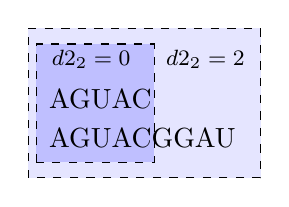
\begin{tikzpicture}
  \draw [fill=blue!10,dashed] (-0.45,0.5) rectangle (2.5,2.4);
  \draw [fill=blue!25,dashed] (-0.35,0.7) rectangle (1.15,2.2);
  \node at (1.0,1.5) {AGUAC\phantom{GGAU}};
  \node at (1.0,1.0) {AGUACGGAU};

  \node at (0.35, 2.0) {\footnotesize $d2_2 = 0$};
  \node at (1.8, 2.0) {\footnotesize $d2_2 = 2$};
\end{tikzpicture}
\caption{Example of difference in distance with window. The distance with the
  window is 0, since the first sequence is a prefix of the other, while the
  distance without the window is 2.}
\label{fig:d2_window_example}
\end{figure}

\subsection{\textsc{K-Dist} algorithm}

This section presents the \textsc{K-Dist} algorithm used in \texttt{klust}.

\textsc{K-Dist} uses a window of length equal to the shortest of the two
sequences being compared. The distance between the substrings in the initial,
leftmost position of the window is calculated using a variant (described below)
of the basic \textsc{d2} algorithm (Algorithm \ref{alg:d2_basic}) described in
section \ref{sec:kmer_distance}. The window then iterates over the longer
sequence, one nucleotide at a time, and calculates the new distance between the
substring of the longer sequence and the shorter sequence.  This calculation is
done using a kind of forward differences method for reducing the calculations
to a few fixed operations for calculating the distance in the next window from
the distance in the current window. This concept is described
in~\cite{hazelhurst}.

\textsc{K-Dist} uses the \emph{Manhattan distance} instead of the Euclidean
distance used in the \textsc{d2} algorithm for calculating the distance between
the two $k$-mer frequency vectors. The Manhattan distance is similar to the
Euclidean distance but with squaring replaced with absolute value and the
square root omitted, i.e.  for $u, v \in \mathbb{Z}^n$,

\begin{equation}
  d_{Manhattan} \eqdef \sum_{i=1}^{n} |u_i - v_i| \;.
\end{equation}

This distance metric was chosen for simplicity, to make the calculation of
distance in subsequent window positions easier, which also improves
performance, and since there is evidence in the literature that the Manhattan
distance generally is preferable to Euclidean distance for high dimensional
distance calculation~\cite{aggarwal}.  % TODO: more about Euclidean being bad

To calculate the distance in the next window position from the distance in the
current window, i.e. advancing the window through the longer of the two
sequences by one character, it is decided which $k$-mers exit and enter the
window, respectively, and then by looking at whether the existing $k$-mer count
in the frequency vector is negative or positive, it can be decided whether the
distance increases or decreased by 2 or whether it stays the same.
Subsequently, the frequency vector is updated to reflect the change in the new
window. Figure \ref{fig:d2_forward_differences} illustrates the idea of a
window and $k$-mers exiting and entering the window:

\begin{figure}[H]
\centering
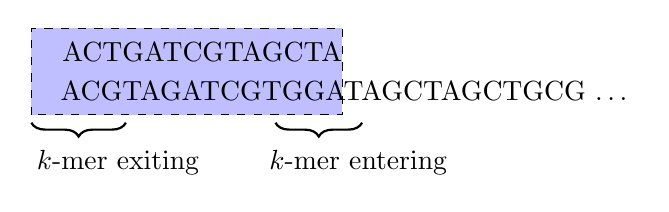
\begin{tikzpicture}
  \draw [fill=blue!25,dashed] (0,0.7) rectangle (3.95,1.8);
  \node at (4.0,1.5) {ACTGATCGTAGCTA\phantom{TAGCTAGCTGCG \dots}};
  \node at (4.0,1.0) {ACGTAGATCGTGGATAGCTAGCTGCG \dots};
  \draw [thick,decorate,decoration={brace,amplitude=5pt,mirror}]
    (0.0,0.6) -- (1.2,0.6) node[midway,xshift=0.5cm,yshift=-0.5cm]
    {$k$-mer exiting};
  \draw [thick,decorate,decoration={brace,amplitude=5pt,mirror}]
    (3.1,0.6) -- (4.2,0.6) node[midway,xshift=0.5cm,yshift=-0.5cm]
    {$k$-mer entering};
\end{tikzpicture}
\caption{Illustration of $k$-mers, where $k=4$, entering and exiting a window.}
\label{fig:d2_forward_differences}
\end{figure}

A distance measure, i.e. not a relative similarity measure, can be difficult to
use for determining sequence similarity since the distance metric is very
dependent on the length of the shortest sequence (the length of the window).

For this reason, the ratio between the Manhattan distance and the maximum
possible distance in the window is used to normalize the distance to a value in
the interval $[0,1]$. Let $w$ denote the size of the window. The corresponding
similarity measure for the Manhattan distance in the window is given by the
following expression:

\begin{equation}
  1 - \frac{d_{Manhattan}(s,t)}{2(w - k + 1)} \label{eq:Manhattan_similarity}
\end{equation}

An alternative notion of similarity, which was the inspiration for the above
similarity measure, is the \emph{Jaccard index}~\cite{jaccard1912}, which is
defined as the size of the intersection of two sets divided by the size of the
union of the sets.  However, the Jaccard index does not take the multiplicity
of the elements into account and therefore it might give a lower sensitivity
than the similarity measure in (\ref{eq:Manhattan_similarity}).

The \textsc{K-Dist} algorithm (Algorithm \ref{alg:K-Dist}) has been implemented
and is used as the distance metric in the \texttt{klust} program. The
$s.substring(i,k)$ method extracts $k$ characters from a string $s$ beginning
at position $i$. The update $cur\_dist$, $\mathtt{kmers}[x]$ and
$\mathtt{kmers}[y]$ statements looks at the values for specific $k$-mers $x$
and $y$ in the $k$-mer vector, increments or decrements the value and updates
the $cur\_dist$ accordingly.

\begin{algorithm}[H]
  \caption{\textsc{K-Dist} algorithm}
  \label{alg:K-Dist}
  \begin{algorithmic}[1]
    \Require{$s$ and $t$ are DNA or RNA sequence, $k \in \mathbb{Z}^+$}
    \Statex
    \Function{K-Dist}{$s, t, k$}
      \State set $s$ to the shorter sequence and $t$ to the longer sequence
      \State initialize map \texttt{kmers} : \texttt{string} $\to$
        \texttt{int} (0 initialized on first access)
      \State $cur\_dist \gets 0$
      \State
      \For{$i \gets 0$ to $\abs{s} - k$}
        \Comment{\parbox[t]{.3\linewidth}{$k$-mer counting}}
        \State $s_i \gets s.substring(i, k)$
        \State $t_i \gets t.substring(i, k)$
        \State update $cur\_dist$, $\mathtt{kmers}[s_i]$ and $\mathtt{kmers}[t_i]$
      \EndFor
      \State
      \State $min\_dist \gets cur\_dist$
      \For{$i \gets 0$ to $\abs{t} - \abs{s}$}
          \Comment{\parbox[t]{.3\linewidth}{No. of windows}}
        \State $kmer_{out} \gets t.substring(i, k)$
        \State $kmer_{in} \gets t.substring(length(s)-k+i+1, k)$
        \State update $cur\_dist$, $\mathtt{kmers}[kmer_{out}]$
               and $\mathtt{kmers}[kmer_{in}]$
        \State $min\_dist \gets min(min\_dist, cur\_dist)$
      \EndFor
      \State
      \State $total \gets 2(length(s)-k+1)$
        \Comment{\parbox[t]{.3\linewidth}{Maximal distance}}
      \State \Return{$(total-min\_dist) / total$}
    \EndFunction
  \end{algorithmic}
\end{algorithm}


\subsubsection{Complexity analysis} \label{sec:k-dist_analysis}

The \textsc{K-Dist} algorithm consists of two loops and a number of constant
operations outside of the loops. In the first loop, the \textsc{K-Dist}
algorithm iterates over the first $|s|-k$ characters, where $|s|$ denotes the
length of the shorter of the two sequences. Each iteration contains only
constant time operations. So far, a running time of $\Theta(\abs{s}-k)$ since
the number of iterations is bounded both from below and from above by
$\abs{s}-k$. This is assuming that the map lookup is $\mathcal{O}(1)$ and that
the $substring$ method is constant time as well, which is the case when strings
are implemented as character arrays, assuming no copying is needed.

In the second loop, \textsc{K-Dist} performs $|t|-|s|$ iterations which each
contains a constant number of constant time operations. This gives a running
time of $\Theta(\abs{t}-\abs{s})$.

This yields a total running time of
\begin{align}
  \Theta(\abs{s}-k) + \Theta(\abs{t}-\abs{s})
  &= \Theta(\abs{s} - k + \abs{t} - \abs{s}) \\
  &= \Theta(\abs{t} - k) \;.
\end{align}

More generally, given two string $s$ and $t$ and $k \in \mathbb{Z}^{+}$, the
\textsc{K-Dist} algorithm has a worst case, average case and best case running
time of $\Theta(\max{\left(\abs{s}, \abs{t}\right)} - k)$.

The space usage of \textsc{K-Dist} depends on the value of $k$ and the $k$-mers
occurring in the sequences, since this affects the size of the \texttt{kmers}
map. The worst case space complexity is $\mathcal{O}\left(4^k\right)$, i.e.
exponential in the value of $k$, however, since $k$ will generally be assumed
to be less than or equal to 8, this is not a problem.

\subsection{Cluster analysis algorithms}

There are several approaches to clustering sequence data. This section
describes different clustering paradigms and it discusses the strengths,
weaknesses and potentials of some of these methods.

\subsubsection{Hierarchical clustering}

\emph{Hierarchical clustering} is typically divided into two types of
clustering algorithms, the agglomerative type that works in a bottom-up manner
and the divisive type that has a top-down approach~\cite{dong}. This section
describes the agglomerative version. In the agglomerative version all sequences
start as leaves in a tree, where the leaves are considered clusters. Each
cluster is then merged together with the closest cluster, thus building a tree,
level for level, until there is only one cluster left. This gives a hierarchy
of the clusters. Alternatively, when the clustering is based on a similarity
threshold, as in this project, the clusters are merged until no more clusters
can be merged. Agglomerative clustering is visualized in Figure
\ref{fig:hierarchical_clustering}.

\begin{figure}[h!]
  \centering
  \def\svgwidth{\columnwidth}
  \import{graphics/}{Hierarchical_Clustering.pdf_tex}
  \caption{Illustration of agglomerative hierarchical clustering. Clusters,
  with objects represented as letters, are merged with nearby clusters based
  on the distance between their positions in the alphabet until there is only
  one cluster.}
  \label{fig:hierarchical_clustering}
\end{figure}

This addresses the question of what is required for a cluster to be ``close''
to another. Besides measuring similarity between sequences with some similarity
metric, a definition for when clusters should be merged is needed. The
following describes different approaches for merging two clusters based on a
similarity threshold.

In the \textit{complete-linkage} approach, all sequences from one cluster must
have a similarity above the threshold to all sequences from the other cluster.
In the \textit{average-linkage} approach, the average similarity between all
pairs of sequences is required to be above the threshold. With the
\textit{single-linkage} approach, at least one sequence from the first cluster
must have a similarity above the threshold to at least one sequence from the
other cluster.

The complete-linkage approach is computationally very heavy as each merge will
take $\mathcal{O}(mn)$ time, where $m$ and $n$ are the sizes of the clusters.
The average-linkage method is equally computationally hard. This is not viable
for a quick clustering algorithm.

The single-linkage approach is often used in sequence
clustering~\cite[pp.~62--63]{dong}. It has the advantage that it can behave
greedily and stop early if a link meets the similarity criterion instead of
calculating all links to find the minimal distance. Though the greedy behavior
can boost performance, it could result in a very rough clustering as two
sequences from the clusters might be very similar while other sequences could
have a very low similarity to each other.

An example of an agglomerative algorithm using the single-linkage approach is
SLINK~\cite{sibson} with complexity $\mathcal{O}\left(n^2\right)$. Another
example, using the complete-linkage approach, is CLINK~\cite{defays}, which is
based on SLINK and also has a complexity of $\mathcal{O}\left(n^2\right)$. As
the naive agglomerative method, both of these algorithms build a distance
matrix and then use row and column operations, but they are optimized to time
complexities of $\mathcal{O}\left(n^2\right)$ instead of
$\mathcal{O}\left(n^3\right)$, where $n$ is the number of sequences.

A running time of $\mathcal{O}\left(n^2\right)$ does not scale well enough for
problem sizes encountered in sequence clustering and it does not need to build
the entire hierarchy. However, with a greedy single-linkage approach and
without building the entire hierarchy, the complexity could be significantly
reduced. The distance matrix itself takes $\mathcal{O}\left(n^2\right)$ time
to create, which is already too much, so this indicates that a heuristic
strategy might be needed.


\subsubsection{Graph-based clustering}

The general framework of graph-based clustering consists of two steps. First
step is to generate a weighted graph from the sequences. The second step, the
clustering step, is to split the graph into subgraphs, which correspond to the
clusters~\cite[pp. 64-65]{dong}.

Consider a graph $G$ with a set of vertices $V$ and a set of edges $E$. In
graph-based clustering, we consider $V$ as the set of sequences and $E$ as the
set of similarity scores. The first step is to calculate all edges $E_{ij}$,
the similarity score between $V_i$ and $V_j$, based on some similarity metric.
If the clustering is based on a similarity threshold, edges that are below the
similarity threshold can be ignored.

There are many variants to the clustering step. E. Hartuv and R. Shamir \\
\cite{hartuv} presents an algorithm that tries to minimize edges that
connect two subgraphs by moving vertices from one subgraph to another.

H. Kawaji \textit{et al.}~\cite{kawaji} presents an algorithm that tries to
maximize the density of edges in a subgraph. This is done by converting the
graph into a simpler graph by removing all edges that are under the similarity
threshold.

Since both algorithms require that the weights of all edges have been computed,
it is already too slow for efficient sequence clustering. If the subgraphs
could be constructed while computing distances, thus avoiding computing all
pairwise distances, the time complexity could be reduced. Both hierarchical and
graph based clustering indicate that a heuristic clustering approach is needed
to obtain the desired performance.


\subsubsection{Greedy algorithm like \texttt{UCLUST}}

The \texttt{UCLUST} algorithm is greedy and is designed so that all member
sequences have similarity greater than or equal to the similarity threshold,
to their centroid.  It works by processing one sequence at a time and
comparing these to the existing centroids. If a match is found, the sequence
is assigned to the cluster of the matching centroid, otherwise it becomes a
centroid of a new cluster. \texttt{UCLUST} attempts to give a clustering
result where each centroid has a similarity under the threshold to all other
centroids, but this is not guaranteed to hold. The reason is that the
algorithm only compares a sequence to a prespecified number of centroids given
by the $max\_rejects$ parameter. It uses the $k$-mer counts to locate centroid
candidates for a match, though how it does it is not very well documented.

The similarity calculations are performed with global sequence alignments as R.
C. Edgar~\cite{usearch_algorithm}  claims that using the word counts to
calculate identity is not sensitive enough. Greedy clustering is illustrated in
Figure \ref{fig:greedy_clustering}.

\begin{figure}[H]
  \def\svgwidth{\columnwidth}
  \import{graphics/}{Greedy_Clustering.pdf_tex}
  \caption{Illustration of greedy clustering. Sequences are processed in the
    order they are read. They either become centroids for new clusters or they
    are assigned to existing clusters.}
  \label{fig:greedy_clustering}
\end{figure}

Greedy clustering can reduce the time complexity as non-centroid sequences are
only handled once. This can also improve space complexity. The time complexity
is dependent on the number of centroids which is typically much lower than the
number of sequences. An efficient search for centroids can reduce the expected
running time to near linear as opposed to the worst case
$\mathcal{O}\left(n^2\right)$ complexity, where $n$ is the number of sequences
(in the case where all sequences become centroids).


\subsection{Naive, greedy clustering algorithm}

A very simple, naive, greedy clustering algorithm, \textsc{Naive-Clust}, has
been implemented and will be described briefly in this section.

Given a list of sequences and an initially empty list of centroids, the
algorithm works by iterating through the sequences and for every sequence, it
iterates through the list of centroids until a match is found or until the end
of the list. If a match is found, the sequences is added to the cluster
represented by the matching centroid, and otherwise the sequences becomes a new
centroid and is appended to the end of the list of centroids.

% TODO: complexity of algorithm
% This running time of this algorithm depends on the number of clusters in the
% output and therefore it might be around $O(c^2)$, where $c$ denoted the
% number of sequences, in the worst case where the number of clusters is equal
% to the number of sequences.  %O(k*(k-1)/2)

% TODO: refer to algorithm and implementation

This approach is not very useful in practice since it is very computationally
expensive in the worst case. The running time of the algorithm is very dependent
on the ordering of the sequences since the centroids will be in the same order
as in the list of sequences (i.e. the list of centroids is a subsequence of the
list of sequences) and if the first number of sequences happens to be good
centroids, which will match a lot of sequences, the algorithm will perform good
since the search for a centroid will end very early. However, if the first
sequences happen to be very dissimilar from the rest of the data, then these
will become centroids and will be compared against on every iteration even
though they might potentially never match anything.

Thus, there is a motivation to try and create more structure in the collection
of centroids, improve the search for a centroid to compare with the query
sequence or improving the ordering of the centroids.

% The problem with this approach is that it is potentially very computationally
% expensive to possible traverse the entire list of centroids for each
% iteration

% TODO: maybe mention the reason for introducing max_rejects and clustering
% algorithm based on greediness


\subsection{\textsc{Simple-Clust} algorithm}

Another clustering algorithm, named \textsc{Simple-Clust}, was developed and
implemented, and will be described in this section. \textsc{Simple-Clust}
tries to address some of the problems with the \textsc{Naive-Clust} algorithm
by imposing more structure on the collection of centroids and by giving up
after some fixed number of comparisons of a given query sequence.

\textsc{Simple-Clust} works by iterating sequentially through the sequences to
be clustered; the $max\_reject$ most frequent $k$-mers for the query sequence
are calculated and for each of these most frequent $k$-mers, a centroid which
has that $k$-mer as the most frequently occurring one (if one such centroid
exists) is compared with the query sequence to check if their similarity is
above the given threshold. The query sequence is assigned to the cluster for
the first centroid that matches the query sequence; if no such centroid is
found, out of the maximum possible $max\_reject$ number of tries, the query
sequence becomes a centroid for a new cluster and is added to the collection of
centroids along with the information about the most frequently occurring
$k$-mer in the sequence. Pseudocode for the algorithm is attached in appendix
\ref{app:simple-clust}.

This algorithm did not perform as well as hoped, in particular for larger $k$
the number of different possible $k$-mers increases exponentially and for e.g.
$k = 6$ and a four letter alphabet, there are $4^6 = 4096$ different $k$-mers
and therefore the lookup in line \ref{alg:line:simple_clust_lookup} of the
algorithm will often be unsuccessful. Additionally, the most frequently
occurring $k$-mer did not appear to be a sufficiently good characteristic for
choosing a centroid that is likely to match, as it is seen from the evaluation
in section \ref{sec:results}. To clarify, the correspondence between the most
frequently occurring $k$-mer of two sequences and the similarity of the
sequences, is evidently not very strong.
% TODO: Maybe move to results?


\subsection{\textsc{K-Clust} algorithm}

This section describes another clustering algorithm that was developed and
implemented, named \textsc{K-Clust}, which looks at the set of $k$-mers
occurring in the query and target sequences and bases the decision of whether
to try comparing or not, on the cardinality of the intersection between these
sets. This way, the search for a likely match is not just determined by the
single most frequently occurring $k$-mer, as with \textsc{Simple-Clust}, but
rather all the occurring $k$-mers, regardless of their count. Additionally, the
centroids are stored in a doubly linked list and whenever a centroid matches a
sequence, that centroid is moved to the front of the list. This makes the
algorithm less sensitive to the ordering of the input sequences. The choice of
the centroids will still be made greedily though, in lack of well-performing
alternatives, but the algorithm should nonetheless be less prone to bad
performance caused by an unlucky ordering of the input sequences. Algorithm
\ref{alg:k-clust} shows pseudocode for the \textsc{K-Clust} algorithm.

The choice of whether to compare a query sequence with a centroid is decided
using the formula
\begin{equation}
  \abs{K(s) \cap K(c)} \geq \abs{K(c)} \cdot id \;
\end{equation}
where $s$ is the query sequence, $c$ is the centroid sequence and $id$ is the
threshold similarity. $K(x)$ denotes the number of $k$-mers in a sequence $x$.
In the \texttt{klust} program this value is hard coded to $k=6$ for performance
reasons.

The idea of moving a matching centroid to the front of the list is, among other
things, inspired by the observation that the results from \texttt{USEARCH} and
\texttt{VSEARCH} often contain a large number of very small clusters and even
singleton clusters, i.e. clusters consisting of just a single sequence.

\begin{algorithm}[H]
  \caption{\textsc{K-Clust}}
  \label{alg:k-clust}
  \begin{algorithmic}[1]
    \Require{$S$ is an array of [DR]NA sequences, $k \in \mathbb{Z}^+$,
            $max\_rejects \in \mathbb{Z}^+$ and $id \in [0,1]$}
    \Statex
    \Function{K-Clust}{$S, k, max\_rejects, id$}
      \State $centroids \gets [~]$ \Comment{initialize empty list of centroids}
      \ForAll{$s \in S$}
        \State $match \gets false$
        \State $rejects \gets 0$
        \State $close\_match \gets \mathtt{NULL}$

        \ForAll{$c \in centroids$}
          \If{$rejects$ \texttt{==} $max\_rejects$}
            \State $break$
          \EndIf

          \State
          \LineComment{$K(x)$: set of $k$-mers in $x$}
          \If{$|K(s) \cap K(c)| \geq |K(c)| \cdot id$}
            \If{\Call{\textsc{K-Dist}}{s, c, k} $ \geq id$}
              \State Add $s$ to cluster represented by $c$.
              \State Move $c$ to the front of $centroids$.
              \State $match \gets true$
              \State $break$
            \EndIf
            \State
            \If{\Call{has\_link}{c} \texttt{AND}
                  \Call{\textsc{K-Dist}}{s, c.link, k} $ \geq id$}
              \State Add $s$ to cluster represented by $c.link$.
              \State Move $c.link$ to the front of $centroids$.
              \State $match \gets true$
              \State $break$
            \EndIf
            \State $rejects \gets rejects + 1$
            \State $close\_match \gets c$
          \EndIf
        \EndFor
        \State
        \If{$\mathtt{NOT}\ match$}  \Comment{add new centroid to list}
          \If{$close\_match$ \texttt{!= NULL}}
            \State $s.link \gets close\_match$
          \EndIf
          \State Prepend $s$ to $centroids$.
        \EndIf
      \EndFor
    \EndFunction
  \end{algorithmic}
\end{algorithm}

An illustration of the method is seen in figure \ref{fig:k-clust}.

\begin{figure}[h!]
  \def\svgwidth{\columnwidth}
  \import{graphics/}{Prioritized_Intersect_Clust.pdf_tex}
  \caption{Illustration of \textsc{K-Clust}. The centroid labeled
    $3$ is pushed to the front of list because it was the latest match to a
    sequence. The centroids labeled $4$ and $5$ has a link to the centroids $0$
    and $1$ respectively because they have been close to matching them.}
  \label{fig:k-clust}
\end{figure}


\subsubsection{Time complexity analysis}

The \textsc{K-Clust} algorithm iterates over the array of sequences $S$, that
is $|S|$ iterations, and for each of these iterations, the algorithms iterates
over the list of centroids $centroids$.

In the worst case, the $centroids$ list will grow with one element in each
iteration of the outer loop, because in the worst case, every sequence will
become a centroid of its own. Thus, the number of iterations in the innner loop
will be the sequence
\[
  1 + 2 + 3 + \ldots + |S| \,,
\]
that is, the $|S|$'th triangular number, which can be expresses as
\begin{equation}
  \frac{\abs{S}\left(\abs{S}+1\right)}{2} \,. \label{eq:triangular_number}
\end{equation}

The inner loop contains a constant amount of work and at most two calls to
\textsc{K-Dist}, which will also be treates as contant time in this context,
since the running time of the clustering algorithm will be expressed in the
number of sequences, rather than the lengths of the sequences. The $K(s) \cap
K(c)$ calculation of the intersection between the two sets of $k$-mers $s$ and
$c$, respectively, will also be treated as constant since it also depends on
the lengths of $s$ and $c$ and not on the number of sequences to be clustered.

Thus, the \textsc{K-Clust} algorithm iterates over the contant amount of work
in the inner loop the number of times expressed in (\ref{eq:triangular_number})
and so the running time is quadratic in the number of sequences, i.e.:
\begin{equation}
  \mathcal{O}\left(\abs{S}^2\right)
\end{equation}

% TODO: analyze space complexity

\section{Theory}
\subsection{Starting out: Levenshtein with dynamic programming}
For a start, a naive version of the Levenshtein distance metric was
implemented, but as expected, this is absolutely useless in any practical
setting, since it does not reuse already calculated results. Therefore, this
was quickly transformed into a dynamic programming solution, which solves
subproblems just once, stores and reuses the intermediate results. This dynamic
programming bottom up solution was however still very slow, yielding a
performance of around 70 comparisons per second. This could most likely be
optimized further, but because of the characteristics of an edit distance
algorithm like Levenshtein and because of the performance requirements for this
project, we choose to not pursue further optimization and instead focus on
other types of algorithms.

\subsection{Simple $d2$ distance}
After learning that the basic Levenshtein algorithm is far too slow for the
problem domain of this project, we turned our attention to the $d2$ distance
metric. The first version of the $d2$ distance metric algorithm is shown in
figure \ref{alg:d2_naive}. This algorithm maintains a single frequency vector,
as a map structure to allow for large $k$ which results in a large number of
possible different $k$-mers. The map is indexed using the lexicographical
position of the $k$-mer. When iterating through the first sequence, $k$-mer
counts are incremented and when iterating through the second sequence, they are
decremented. Finally all the frequencies are squared and the square root of the
sum is returned, corresponding to the Euclidean distance between frequency
vectors for the two sequences.

\begin{algorithm}
  \caption{Naive \textsc{d2} distance metric}
  \label{alg:d2_naive}
  \begin{algorithmic}[1]
    \Require{$s$ and $t$ are DNA or RNA sequences and $k \in \mathbb{Z}^+$}
    \Statex
    \Function{d2}{$s, t, k$}
      \State initialize \texttt{freq\_map}
      \For{$i \gets 0$ to $length(s) - k$}
        \State freq\_map[index\_of\_kmer(s.substring(i, k)]\texttt{++}
      \EndFor
      \For{$i \gets 0$ to $length(t) - k$}
        \State freq\_map[index\_of\_kmer(t.substring(i, k)]\texttt{--}
      \EndFor
      \State $total \gets 0$
      \ForAll{$e \in$ freq\_map}
        \State $total \gets e.value^2$  \Comment{calculate the Euclidean distance}
      \EndFor
      \State \Return $\sqrt{total}$
    \EndFunction
  \end{algorithmic}
\end{algorithm}


\subsection{$d2$ distance with windows and Jaccard index}
The current version of the $d2$ distance function uses the concept of a
\emph{window}, of a certain length, that iterates over the sequences and
calculates distances between the substrings in each window. This calculation is
done using a kind of forward differences method for reducing the calculations
to a few fixed operations for calculating the distance in the next window from
the distance in the current window. This concept is described in
\cite{hazelhurst}.

The algorithm presented here uses a window size equal to the length of the
shortest of the two sequences. Let $|s|$ be the length of the shortest of the
two sequences. To begin with the, the $k$-mers in the first $|s|$ characters of
each sequence are counted and the \emph{Manhattan} distance between these two
frequency vectors is calculated.

The Manhattan distance is simply the Euclidean distance where squaring is
replaced with absolute value and the square root is omitted, i.e. for
$u, v \in \mathbb{Z}^n$,

\begin{equation}
  d_{Manhattan} \eqdef \sum_{i=1}^{n} |u_i - v_i| \;.
\end{equation}

This distance is the distance between the subsequences in the first position of
the window. To calculate the distance in the following window, i.e. advancing
the window through the longer of the two sequences by one character, it is
decided which $k$-mers exit and enter the window, respectively, and then by
looking at whether the existing $k$-mer count in the frequency vector is
negative or positive, it can be decided whether the distance increases or
decreased by 2 or whether it stays the same. Subsequently, the frequency vector
is updated to reflect the change in the new window. The following illustrates
the idea of a window and $k$-mers exiting and entering the window:

\begin{verbatim}
      |---- window ----------|
      ACTGATCGTAGCTAGCTAGTGTTG
      ACGTAGATCGTGGATGGCTGATCGTAGCTAAGCTTAGCTGATCG.....
      ^^^^                 ^^^^
      k-mer exiting        k-mer entering
\end{verbatim}

The Manhattan distance can be hard to use in practice, because it is very
dependent on the length of the shortest sequence (the length of the window),
the concept of the \emph{Jaccard index}, or the \emph{Jaccard similarity
coefficient}, is used to ``normalize'' the distance to a value in the interval
$[0,1]$.

The Jaccard index of two sets $A$ and $B$ is defined as follows:
\begin{equation}
  J(A, B) \eqdef \frac{|A \cup B| - |A \cap B|}{|A \cup B|}
\end{equation}
 % TODO:  maybe actually Jaccard distance; maybe add citation

In the context of $k$-mer frequencies, the union can be interpreted as the
total number of $k$-mers in the window in the two sequences, and the
intersection as the Manhattan distance in the window.


\section{Results and evaluation} \label{sec:results}

\subsection{Overview of datasets used for testing}

A couple of different datasets will be used for testing and evaluating the
implementation of the distance metrics and clustering algorithms presented in
section \ref{sec:methods}. These datasets will be briefly presented in this
section.

\begin{description}
  \item[\texttt{SILVA}] \hfill \\
    The dataset \texttt{SILVA\_119\_SSURef\_tax\_silva.fasta} has a size of
    around 2.3GB and contains $1,583,830$ RNA sequences of average length
    1415.46, minimum length 900, maximum length 3845 and median length 1389.
    The data looks very clean and contains very few characters aside from the
    actual RNA bases, i.e. only very few 'R', 'N', 'K' etc.  characters.

  \item[\texttt{RDP}] \hfill \\
    The dataset \texttt{RDP\_Pro\_Full.sort.fna} has a size of around 3.5 GB
    and contains $3,019,928$ DNA sequences of average length 1044.19, minimum
    length 400, maximum length 2922 and median length 1132.
\end{description}

Various statistics about the datasets are shown in figure \ref{fig:data_stats}.

\begin{figure}[H]
  \centering
  \begin{tabular}{c | c | c | c | c | c }
    Dataset        & Sequences & Avg. len. & Min. len. & Max. len. & Median len.\\
    \hline
    \texttt{SILVA} & 1,583,830 & 1415.46   & 900       & 3845      & 1389       \\
    \texttt{RDP}   & 3,019,928 & 1044.19   & 400       & 2922      & 1132       \\
  \end{tabular}
  \caption{Various information about the different datasets.}
  \label{fig:data_stats}
\end{figure}

% SILVA:
% avg_len:       1415.46
% min_len:       900
% max_len:       3845
% median:        1389
% dirty:         350055
% dirty/sum_len: 0.000156146

% RDP:
% avg_len:       1044.19
% min_len:       400
% max_len:       2922
% median:        1132
% dirty:         2518801
% dirty/sum_len: 0.000798764


\subsection{Testing the distance metric on altered sequences}
\label{sec:altered_sequences}

% TODO: can't get this crap right....
%A few different sets of highly similar sequences were synthetically constructed
%from real data and used in the evaluation the distance metric.
%
%A sequence was randomly chosen from \texttt{SILVA} and four sets, each
%containing ten copies of this sequence, were made. For each sequence in the
%first two sets, a list of random indices in the sequence was generated and in
%each of these indices in the sequence, a substitution for a different, randomly
%chosen nucleotide was made. For the first set, this list was of legnt

Two different sets of highly similar sequences was constructed from a real
world sequence from \texttt{SILVA} and this was used in the evaluation of the
distance metric.

One sequence was chosen, 10 copies of this sequences were made and to each of
these copies, a few alterations were made. In the first set, a list of random
indices in the sequence were generated and in each of these indices in the
sequence, a substitution for a different, randomly chosen nucleotide was made.
This was done twice, for different degrees of alteration, and the number of
alterations was equal to respectively 1\% and 2\% of the length of the
sequence.

In the second set, the same number of alterations to individual nucleotides
were made, but in this case they were grouped into alterations of substrings of
length 5 (one such group being of length less than 5 if the number of
alterations were not a multiple of 5).

For illustration, figure \ref{fig:alterations} shows an original sequence in
the first line, the single edits alterated sequence in the second line and the
chunk alterated sequence in the third line.

\newcommand{\tc}[1]{\textcolor{red}{#1}}
\begin{figure}[H]
  \centering
  \texttt{AAAAAAAAAAAAAAAAAAAAAA} \\
  \texttt{AAAAA\tc{T}AA\tc{C}AAAA\tc{G}AAAA\tc{T}AAA} \\
  \texttt{AAA\tc{TC}AAAAAAAAAA\tc{GG}AAAAA}
  \caption{Two types of alterations to sequences: the original sequence in the
    first line, single edit alterations in the second line and chunks of edits
    in the third line.}
  \label{fig:alterations}
\end{figure}

The $k$-mer based distance metric, presented in section
\ref{sec:kmer_distance}, is expected to be more sensitive to a number of
individual changes than to the same number of changes made in chunks. This test
serves to confirm this expectation and to give an insight into the change in
$k$-mer distance when performing a controlled number of edits.

The similarities between the original sequence from \texttt{SILVA} and the 10
altered sequences, for the four different types of alterations, are shown in
figure \ref{fig:altered_seqs_similarities}.

\begin{figure}[H]
  \centering
  \begin{tabular}{c|c||c|c}
    \multicolumn{2}{c||}{single edits}  & \multicolumn{2}{c}{chunk edits} \\
    \hline\hline
    1\%   &   2\%                   &   1\%   &   2\% \\
    \hline
    0.944   & 0.889                     & 0.980     & 0.960 \\
    0.947   & 0.887                     & 0.979     & 0.960 \\
    0.944   & 0.893                     & 0.979     & 0.960 \\
    0.941   & 0.902                     & 0.979     & 0.961 \\
    0.944   & 0.894                     & 0.979     & 0.958 \\
    0.947   & 0.894                     & 0.979     & 0.958 \\
    0.941   & 0.895                     & 0.982     & 0.958 \\
    0.945   & 0.891                     & 0.979     & 0.961 \\
    0.945   & 0.889                     & 0.979     & 0.958 \\
    0.946   & 0.897                     & 0.981     & 0.958
  \end{tabular}
  \caption{Similarity measures for 1\% and 2\% single edits, respectively,
    and 1\% and 2\% chunk edits, respectively, to 10 copies of a single
    sequence.}
  \label{fig:altered_seqs_similarities}
\end{figure}

As expected, the single edits result in a lower similarity that the
corresponding chunk edits. This is because five individual changes will affect
the count of up to $5 \cdot k$ $k$-mers, while five changes in sequence will
only affect up to $4+k$ $k$-mers.


\subsection{Constructing a synthetic dataset}

A synthetic dataset was constructed for evaluating the clustering algorithm's
ability to find the right clusters in a dataset with a clearly correct,
expected clustering output.

A set of sequences was chosen from \texttt{SILVA} by clustering with a
similarity threshold of $0.5$ and choosing the 20 first centroids from the
result. These centroids were confirmed to be dissimilar by calculating the
distance matrix for the sequences and checking that all the similarities were
below $0.5$.

For each of these sequences, 10 copies were made and chunks of changes were
made to these as described above in section \ref{sec:altered_sequences}. This
should yield a set of 210 sequences with 20 expected clusters, which each
should contain sequences with similarities of approximately $0.98$ for $1\%$
changes and approximately $0.96$ for $2\%$ changes.


\subsection{Evaluating distance metric}

To evaluate our implementation of the $k$-mer distance using windows and the
Jaccard index, the Levenshtein distance was used as reference. Since the
Levenshtein distance does not produce values between $0$ and $1$, the Jaccard
index was used here as well.

In figure \ref{fig:Levenshtein_vs_Kmer} is three scatter plots with the
Levenshtein distance on the $y$-axis and our version of the $k$-mer distance on
the $x$-axis. The three plots are with $k=4, k=6$ and $k=8$.

The scatter plots gives an indication about when and how sensitive our
implemented distance metric is. We want the distance to be as close as possible
to a linear function without too much variance, but not necessarily to the line
$y=x$. If it can be expressed linearly it means there is a correlation between
the two. If it can be expressed as $y=x$ (or close) it means that they measure
the same distance which is favourable.

When $k=4$ there is a linear relation when the identity $I>0.9$, but when
$I<0.9$ there is too much variance in the points from any linear function.

With $k=6$ there seems to be a linear relation when $I>0.8$. When $I<0.8$ there
is more variance though less than when $k=4$.

When $k=8$, it is very similar to $k=6$. It seems there is a linear relation
for $I>0.8$ again and when $I<0.8$ the variance is greater.

\begin{figure}
  \begin{subfigure}[b]{0.5\textwidth}
    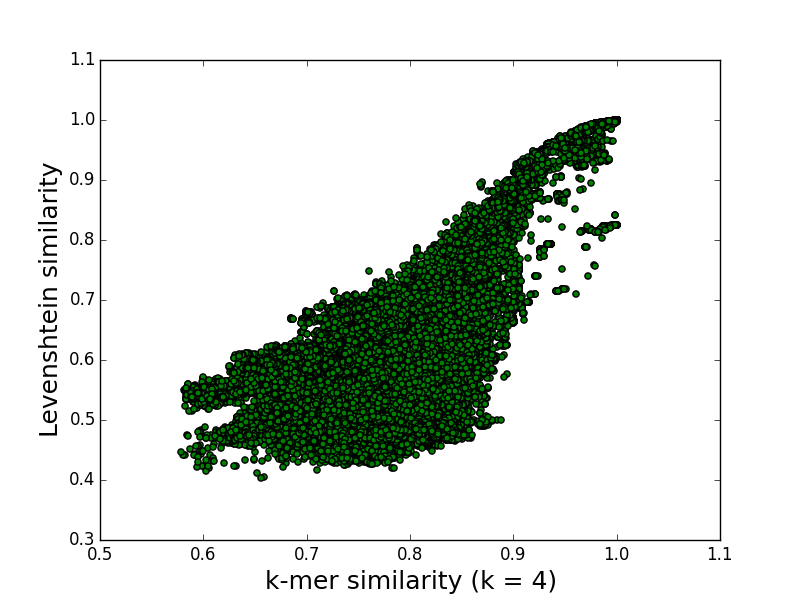
\includegraphics[scale=0.34]{graphics/k4.png}
  \end{subfigure}
  \begin{subfigure}[b]{0.5\textwidth}
    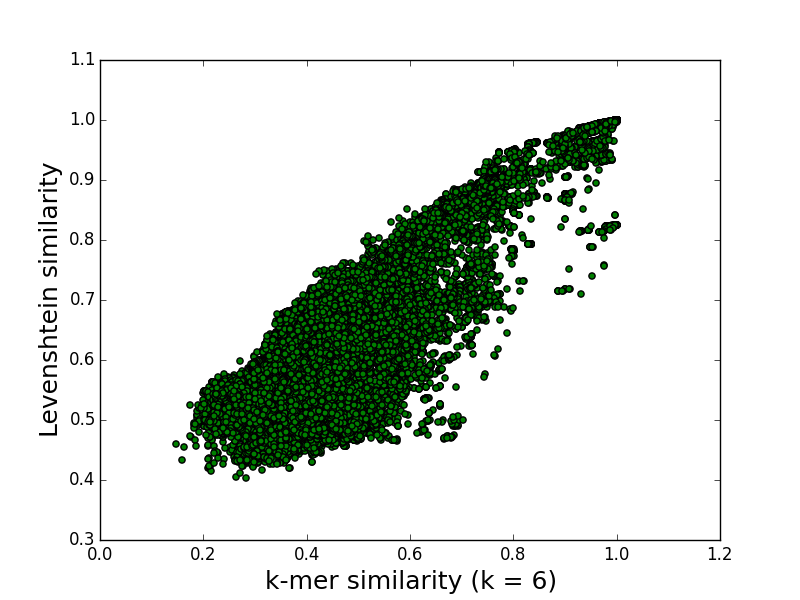
\includegraphics[scale=0.34]{graphics/k6.png}
  \end{subfigure}

  \centering
  \begin{subfigure}[b]{0.5\textwidth}
    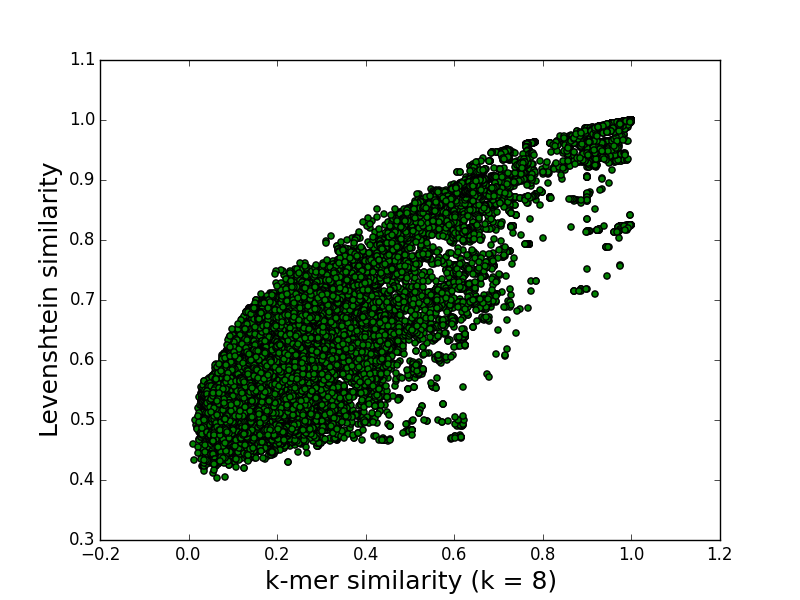
\includegraphics[scale=0.34]{graphics/k8.png}
  \end{subfigure}
  \caption{Comparison of Levenshtein distance and our implementation of the
  $k$-mer distance using windows and Jaccard index.}
  \label{fig:Levenshtein_vs_Kmer}
\end{figure}


\subsection{Comparing with UCLUST on real life data}
% Testing USEARCH 32-bit on real data
% Testing clustering algorithm with d2 distance and comparing performance to
% USEARCH.
Running \texttt{USEARCH} on the file
\texttt{SILVA\_119\_SSURef\_tax\_silva.fasta} after it is sorted with
parameters \texttt{-clust\_smallmem} and \texttt{-id 0.95} produces the
following output

\begin{figure}[H]
\begin{lstlisting}[style=output-style]
28:39 1.1Gb  100.0\% 117205 clusters, max size 83904, avg 13.5
      Seqs  1583830 (1.6M)
  Clusters  117205 (117.2k)
  Max size  83904 (83.9k)
  Avg size  13.5
  Min size  1
Singletons  67410 (67.4k), 4.3\% of seqs, 57.5\% of clusters
   Max mem  1.1Gb
      Time  28:41
Throughput  920.3 seqs/sec.
\end{lstlisting}
  \caption{Output from \texttt{USEARCH} clustering.}
  \label{fig:uclust_silva}
\end{figure}

Running our implementation of the same file but unsorted and with
\texttt{id=0.9, k=6} og \texttt{max\_rejects=8} produces the following

\begin{figure}[H]
\begin{lstlisting}[style=output-style]
Reading 1583830 sequences...
Finished reading:
Time: 24.8109 sec.
Seqs/sec: 63836
Clustering 1583830 sequences...
26.4602
# of clusters: 1364006
Finished clustering:
Time: 187.355 sec.
Throughput: 8453.63seqs/sec.
\end{lstlisting}
%TODO caption and label?
\end{figure}

Even though the \texttt{id}'s does not represent the same threshold due to it
being two different distance metrics we do get a lot more clusters. Running
it with similar \texttt{id}'s produces almost the same amount of clusters, so
the problem lies in the way we choose our centroids we compare a query
sequence with.

Our implementation, however, is faster by a factor of $10$. This can be
attributed to our choice of distance metric.

%Possibly things to look into: confusion matrix, Rand index, normalized
%mutual information (article: Comparing Clusterings - An Overview).


\subsection{Evaluating clustering algorithm on real data}

This section describes one way of evaluating the
\textsc{Prioritized\_Intersect\_Clust} algorithm on real \texttt{RNA} data
(\texttt{SILVA}) using multidimensional scaling (MDS) and t-distributed
Stochastic Neighbor Embedding (t-SNE). This was done using \texttt{Python} with
\texttt{matplotlib} and \texttt{scikit-learn}.

One example of this
multidimesional scaling on the distance matrix for the first 500 sequences of
\texttt{SILVA} is shown in figure \ref{fig:mds_tsne}. The centroids found using
the clustering algorithm \textsc{Prioritized\_Intersect\_Clust}, with similarity
threshold 0.85, $max\_rejects$ 8 and $k$ 6, are pinpointed in the plot and
labeled with the numbers of the sequences in the order they were read.

\begin{figure}[h!]
  \centering
  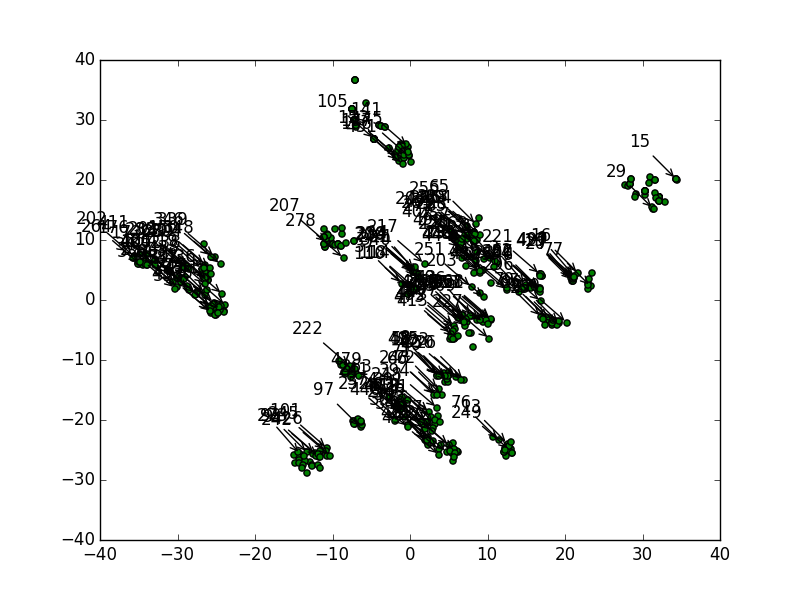
\includegraphics[width=\textwidth]{graphics/MDS_t-SNE_SILVA_500.png}
  \caption{Multidimensional scaling with annotations on centroids.}
  \label{fig:mds_tsne}
\end{figure}


\subsection{Results}
\begin{figure}[H]
  \centering
  \begin{tabular}{ c | c }
    Metric                                        & Comparisons/second      \\
    \hline \hline
    Dynamic programming (bottom up) Levenshtein   & $\sim$ 70               \\
    \hline
    d2-distance with window, $k=4$                & $\sim$ 73000            \\
    \hline
    d2-distance with window, $k=6$                & $\sim$ 63000            \\
    \hline
    d2-distance with window, $k=8$                & $\sim$ 24000            \\
  \end{tabular}
  \caption{Performance of different distance metrics.}
\end{figure}

\begin{figure}[H]
  \centering
  \begin{tabular}{ p{12em} | c | c }
    Method  & Throughput/second   & \# of clusters \\
    \hline \hline
    \textsc{Simple\_Clust}, $k=4$,
    $max\_rejects=8$, $id=0.97$     & $\sim$ 11,400  & 444,654  \\
    \hline
    \textsc{Simple\_Clust}, $k=5$,
    $max\_rejects=8$, $id=0.97$     & $\sim$ 10,700  & 461,266  \\
    \hline
    \textsc{Simple\_Clust}, $k=6$,
    $max\_rejects=8$, $id=0.97$     & $\sim$ 9,575   & 470,516  \\
    \hline
    \textsc{Simple\_Clust}, $k=7$,
    $max\_rejects=8$, $id=0.97$     & $\sim$ 6,350   & 474,463  \\
    \hline
    \textsc{Simple\_Clust}, $k=8$,
    $max\_rejects=8$, $id=0.97$     & $\sim$ 2,750   & 475,465  \\
  \end{tabular}
  \caption{Performance of different clustering methods and different $k$-mer
  sizes. Sequence data:
           \texttt{RDP\_Pro\_Full\_sort.fna}. Count: 500,000. Throughput
           specifies the number of sequences clustered per second (including
           results output to file), but excludes reading the input file.}
\end{figure}

\section{Conclusions and future work}

\subsection{Current status and plan for the rest of the project}

At this point in the project, we have described and implemented a reasonably
fast distance metric, which might be able to compete with other existing
solutions, e.g. \texttt{UCLUST}, depending on the clustering algorithm used
with the distance metric. There is still room for improvement, however, for
instance we plan to implement storage of $k$-mer frequency vectors together
with the centroids such that these can be reused in subsequent similarity
calculations.

Additionally, there can be made more checks for the possibility of stopping a
comparison early, if it is already known that it will fail.

While the distance metric implementation can be improved we also need to keep
it sensitive. Changing the distance metrics to improve speed could mean a
drawback for its sensibility. We also plan to investigate alternative methods
to locate centroid candidates as the current implementation does not provide
good results.



\newpage
\addcontentsline{toc}{section}{References}
\bibliography{report}
\bibliographystyle{plain}

\newpage
\appendix
\section{Algorithms}

\subsection{Bottom-up dynamic programming Levenshtein algorithm}
\label{app:levenshtein_algorithm}

\begin{algorithm}
  \caption{Bottom-up dynamic programming Levenshtein algorithm}
  \label{alg:levenshtein}
  \begin{algorithmic}[1]
    \Require{$m$ and $n$ are DNA or RNA sequences}
    \Statex
    \Function{levenshtein}{$m, n$}
      \State Initialize arrays \texttt{p} and \texttt{q}
      \For{$i \gets 0$ to $length(m)$}
        \State p[i] = i
      \EndFor
      \For{$i \gets 0$ to $length(n)-1$}
        \State q[$0$] = $i+1$
        \For{$j \gets 0$ to $length(m)-1$}
            \If{m[$j$] = n[$i$]}
              \State cost = 0
            \Else
              \State cost = 1
            \EndIf
            \State q[$j+1$] = min(q[$j$] + $1$, p[$j+1$] + 1,          
            p[$j$] + cost)
        \EndFor
        \For{$j \gets 0$ to $length(m)$}
            \State p[$j$] = q[$j$]
        \EndFor
      \EndFor
    \State \Return q[$length(m)$]
    \EndFunction
  \end{algorithmic}
\end{algorithm}


\end{document}
